%% 
%% 
%% 

% \chapter{Related Work and Background}
% \label{cha:RelatedWorks}

\section{Introduction}
\label{sec:intro}

Quantitative trading algorithms using machine learning and data
mining technologies have been raising much interest these years
\cite{fasanghari2010design,cremers2009active,hsu2011hybrid,leung2013discovering}.
Machine learning algorithms leveraging Big Data and novel
hardware can form the basis for effective stock price movement
reasoning and artificial intelligent trading decision making.
This gives traders a wild range of new insights and opportunities
to combine prior knowledge of financial market with non-observable
information into trading strategies.

Price movement prediction is an extremely difficult optimization
and mathematical modeling problem regarding its basis in
stochastic movements and complex dynamic system.

Since the beginning of 2017, some blue chip stocks which have low
valuations, solid market positions and steady earnings have been
in hot pursuit of funds, with prices rapidly rising up. However,
according to the Wind Financial Terminal, by May 25, 2017, more
than 80\% of stocks have been fallen, and specifically, the
number of stocks which have declined by more than 20\% has been
near 1200, accounting for 40\% of stocks (rule out the sub-new
stocks). These phenomena show fierce differentiation of China’s
stock market.

Corresponding to the A share market, due to the great difference
of configuration between industry and single stock, the
performances of active funds also suffered a period of great
division. The prices of funds which heavily invested in the blue
chip stocks were driven up, boosting the yields and hitting new
highs. But meanwhile, the net worth scale of some funds seriously
shrank whose heavy warehouse stocks are those of SME stock market
or defense industry plate, resulting heavy fall of multiple
funds. Similarly, the performances of public enlisting funds
represent extreme divergences.

Price prediction is a significantly difficult optimization and
mathematical modeling problem regarding its basis in stochastic
movement and complex dynamic system. The algorithms which can
accurately predict the fluctuation of stock price bring huge
underlying income for fund managers and financial investors.
Machine learning algorithms leveraging big data are able to form
the basis for effective stock price prediction and trading
decision making, so quantitative trading algorithms using machine
learning and data mining technologies have been raising much
interest these years [7, 8, 12, 18]. Consequently, a wild range
of new insights and opportunities are provided for the traders to
combine prior knowledge of finance with non-observable
information.


In this paper, we demonstrate the application of machine learning
techniques together with fundamental financial analysis in
trading strategies development. We model the complex
relationships between companies by using the famous Markov Random
Fields (MRFs) and leveraging the structure information implied in
those relationships by Structural Support Vector Machine (SSVM).
In order to encode complex consistency information between
stocks, we trained two Gaussian Mixture Models (GMMs) (one for
positive movement, one for negative movement). The cutting-plane
algorithm was developed in favor of making the learning problem
of SSVM tractable and convergence.

Key contributions in this paper are:

(i) Encoding consistency information between collaborating
companies using GMMs.

(ii) Modeling stock price movements using MRFs and SSVM.

The remainder of this paper is organized as follows. The next
section discusses three main problems we focus on: energy
function, inference and learning problem. Then we introduce our
energy function formulation together with our exact inference
using st-min-cut algorithm. The following section describes our
MRFs with unary and pairwise potential functions' quadratic
programming formulation under the max-margin framework (SSVM) and
the cutting-plane algorithm for solving SSVM. In the last section
we describe our experiment configuration and show the improvements
made by our algorithm by comparing with previous works. We also
give some real-world application insights in that section by back
testing a trading strategy developed using our algorithm.

\section{Related Work and Background}
\label{sec:RelatedWorks}
\subsection{Markov Random Fields}
\label{sec:MRF}
\emph{Markov Random Fields} are also known as \emph{undirected
  graphical model} can be seen as a regularized joint
log-probability distribution of arbitrary non-negative functions
over a set of maximal cliques of the
graph~\cite{bishop:2006:PRML}. Let $C$ denotes a maximal clique
in one graph and $\by_C$ denotes the set of variables in that
clique. Then the joint distribution can be written as:
\begin{align}
  p(\by)=\frac{1}{Z}\prod_{C}{\Psi_C(\by_C)}
\end{align}
\noindent where $\Psi$ is called \emph{potential functions} which
can be defined as any non-negative functions and
$Z=\sum_{\by}\prod_{C}{\Psi_C(\by_C)}$ which is a normalization
constant. To infer labels which best explains input data set, we
can find the \emph{maximum a posteriori} (MAP) labels by solving
$\by^*=\argmax_{\by}p(\by)$. Because potential functions are
restricted to be non-negative, it gives us more flexible
representations by taking exponential of those terms. Thus the
joint distribution becomes:
\begin{align}
  p(\by)=\frac{1}{Z}exp(-\sum_{C}{E_C(\by_C)})
\end{align}
\noindent where $E$ is called \emph{energy functions} which can be
arbitrary functions. Therefore, \emph{maximum a posteriori}
problem is equivalent to \emph{energy minimization} problem,
which is also known as \emph{inference}:
\begin{align}
  \by^*& =\argmax_{\by}p(\by)=\argmax_{\by}\big(exp(-\sum_{C}{E_C(\by_C)})\big)\notag
  \\&=\argmin_{\by}(\sum_{C}{E_C(\by_C)})
\end{align}
To optimize the performance we can also consider a weighted
version of energy functions. In order to do this we can decompose
energy functions over nodes $\N$, edges $\E$ and higher order
cliques $\C$~\cite{Szummer:ECCV08} then add weights on them
accordingly. Let $\bw$ be the vector of parameters and $\phi$ be
arbitrary feature function, then the energy can be decomposed as
a set linear combinations of weights and feature vectors:

\begin{align}
  \label{eq:energyfunction_UPH}
  E(\by;\bw)=&\sum_{i\in \N}{\bw_i^U\phi^U(\by_i)}+
               \sum_{(i,j)\in \E}{\bw_{ij}^P\phi^P(\by_i,\by_j)} \notag \\
               &+\sum_{\by_C\in \C}{\bw_C^H\phi^H(\by_C)}
\end{align}

\noindent where $U$ denotes \emph{unary} terms, $P$ denotes
\emph{pairwise} terms and $H$ denotes \emph{higher order} terms
(when $|C|>2$ namely each clique contains more than two
variables).

A weight vector $\bw$ is more preferable if it gives the
ground-truth assignments $\by_t$ less than or equal to energy
value than any other assignments $y$:

\begin{align}
E(y_t,w)\leq E(y,w)~ \text{,~}\forall y \neq y_t
\text{,~} y\in \Y
\end{align}


Thus the goal of \emph{learning} MRFs is to learn the parameter
vector $\bw^*$ which returns the lowest energy value for the
ground-truth labels $y_t$ relative to any other assignments
$y$~\cite{Szummer:ECCV08}:

\begin{align}
\bw^* = argmax_{\bw}(E(y_t,w)-E(y,w))~ \text{,~}\forall y \neq y_t
\text{,~} y\in \Y
\end{align}

So far we have introduced three main research topics of MRFs:
definition of \emph{energy function} (potential functions),
\emph{inference} problem (MAP or energy minimization) and
\emph{learning} problem.

As for energy function, our work focus on a generalization of
k-means clustering known as Gaussian Mixture Models to
incorporate information about the covariance structure of the
data as well as the centers of the latent Gaussians. The
grabcut~\cite{Rother:SIGGRAPH04} algorithm is used to train GMMs
and the final results are used to construct the unary terms. For
pairwise terms, we use the Potts model introduced by
\citename{Kohli:CVPR07} to encode pairwise consistency. The
\emph{inference} problem is solved by using a
graph-cut~\cite{Boykov:ICCV99, Boykov:PAMI04} algorithm and the
max margin framework~\cite{tsochantaridis2005large} has been
addressed to learn parameters of the energy function.

\section{Energy function and exact inference}
\label{sec:energy_and_inference}


\subsection{Construction of MRF (stocks' relationship) graph}
\label{sec:con_stock_graph}

As a complex system, the stock market is full of abundant of
variables which affect the value of shares to rise or fall.
Specifically, if some companies collaborate in their business,
their stock prices even will consistently fluctuate. To
concretely capture such kind of relationship among different
companies, we can unfold it with an undirected graph (MRFs). Each
node in the graph represents a single company, and the edge
between a pair of nodes implies that the two related companies
work in close collaboration.

In this paper, we will select the 300 stocks covered by SHANGHAI
SHENZHEN 300 INDEX (CSI 300) as the experiment subjects (the data
supplied by Wind Financial Terminal). Since collaboration exists
among many corporations, if inference is decided by a
message-passing algorithm (the complexity is exponential in the
tree-width of the graph), the problem will become intractable. As
mentioned above, we are capable of using minimum cuts to solve
inference queries in polynomial time to figure out the
collaboration and competition relationship among the 300
companies through \emph{sougo.com} search engine:

1. Company A-Company B collaboration

2. Company A-Company B competition

To reduce the probability of mistakes in falsely judging the
relationship, we set a threshold value as 1.5: if the number of
results searching with the first query is 1.5 times bigger than
that with the second one, we assume that the collaboration exists
between the company A and B. Correspondingly, an edge will be
used to connect the related nodes in the MRFs. Our spider code
and graph data are available on Github
\url{https://github.com/spacegoing/sogou_spider}.

The unary terms are measured using GMMs and pairwise terms are
measured using Potts model, requiring the SSVM to learn the
labeling from the feature vectors at the nodes.

\subsection{Configuration of Energy Function}
\label{sec:grabcut}

\begin{figure}[b]
  \centering
  
\includegraphics[width=1\linewidth]{RelatedWorks/figures/grabcut_task.png}
  \caption{\label{fig:grabcut_example} Picture on the left is
    the original picture. Picture
    on the middle is a user defined mask. The task is to extract
    foreground pixels within that rectangle. On the right is the
    ground truth foreground.}
\end{figure}

In this section we described the configuration of our energy
function. We mainly introduce the \emph{GrabCut} algorithm which
we use to generate our unary terms. The \emph{Potts model} is
used as our pairwise terms. Thus our energy function can be
written as:
\begin{align}
  \label{eq:energyfunction_UP}
  E(\by;\bw)=\theta^U\sum_{i\in \N}{\bw_i^U\phi^U(\by_i)}+
  \theta^P\sum_{(i,j)\in \E}{\bw_{ij}^P\phi^P(\by_i,\by_j)}
\end{align}
\noindent where $\theta^U$ and $\theta^P$ are parameters to be
optimized.

The \emph{GrabCut} algorithm was proposed
by~\citename{Rother:SIGGRAPH04} in order to solve background
foreground segmentation problem (see
figure~\ref{fig:grabcut_example}). They first defined MRFs over
an labeled image and then use
\emph{graph-cuts}~\cite{Boykov:ICCV01} method to do the
inference. The equivalence of the labeled image in our work is
the stocks relation graph described in
section~\ref{sec:con_stock_graph}. We use two of their
contributions: estimating color distribution (foreground and
background) using \emph{Gaussian Mixture Models} (GMMs) and an
\emph{EM} like two-step algorithm to train their model.

Suppose there are $N$ stocks in our stocks graph. In order to
construct MRFs, we first defined an energy
function~\eqref{eq:energyfunction_UPH} with unary and pairwise
terms:

\begin{align}
  \label{eq:grabcut_energy}
  G(\alpha, \bk, \btheta, \bz) = 
  \sum_{i\in \N}{\psi^U(\alpha_i, \bk_i, \btheta, \bz_i)}+
  \sum_{(i,j)\in \E}{\psi^P(\alpha_i,\bz_i)}
\end{align}
where $i$ is the index of pixels, $\alpha \in {0,1}$ is the label
for pixel $i$. $0$ is for the background and $1$ is for the
foreground. $\bz$ denotes the pixel vector in RGB color space.
$\bk$ and $\btheta$ are all parameters vectors.

\begin{algorithm}[tb]
  \begin{algorithmic}[1]
    \REPEAT
    \STATE{\emph{Assign GMM components} to stocks: \\
      $\bk_i^*=\argmin_{\bk_i}\psi^U(\alpha_i, \bk_i, \btheta,
      \bz_i)$}
    \STATE{\emph{Learn GMM parameters} from data z:\\
      $\btheta=\argmin_{\btheta}\sum_{i\in \N}{\psi^U(\alpha_i, \bk_i, \btheta, \bz_i)}$}
    \STATE{\emph{Estimate segmentation}: graph-cuts inference:\\
      $\min_{\alpha}\min_{\bk}E(\alpha, \bk, \btheta, \bz)$}
    \UNTIL{convergence}
  \end{algorithmic}
  \caption{\label{alg:grabcut} GrabCut training algorithm}
\end{algorithm}

In our configuration, we use the graph described in
section~\ref{sec:con_stock_graph} in replacement of the image.
Each node in the graph represents a stock instead of pixel and
the edge between stocks represents their pairwise relationship.
The label $\alpha \in {0,1}$ equals $1$ when the stock price has
a positive movement, and vice versa. $\bz$ denotes the stock's
market price vector instead of pixel's RGB value

\begin{align}
  \label{eq:feature_vector}
  \bz =
  \begin{bmatrix}
    \text{open} \\
    \text{high} \\
    \text{low} \\
    \text{close} \\
    \text{volume} \\
    \text{macd}_5 \\
    \text{macd}_{10} \\
    \text{kdj}_9
  \end{bmatrix}
\end{align}

\noindent Other parameters are the same with their configurations.

The \emph{Gaussian Mixture Models} (GMMs) with $K$ components
(typically $K=5$) is used for generating unary terms. Two GMMs,
one for positive movement and one for negative movement, are
jointly trained by the algorithm.
$\bk={\bk_1,\dots,\bk_i,\dots,\bk_N}$ with $\bk_i\in 1,\dots,K$
assigns each stock (node) $i$ to a unique GMMs component. The
component is either belonging to positive movement's GMMs or
negative movement's GMMs, which is depended on the label
$\alpha_i\in {0,1}$. $\btheta$ is the parameter vector which
contains parameters of standard GMMs plus \emph{mixture weighting
  coefficients}~\cite{Rother:SIGGRAPH04}.

The pairwise function $\psi^P$ in \eqref{eq:grabcut_energy} is
defined as a smoothness indicator which measures both feature
vector (stock price vector) and spatial distances (graph
distances) simultaneously. It is used to encourage coherence of
similar pixel pairs. Energy function~\eqref{eq:grabcut_energy}
was later used to construct an \emph{st min-cut} graph which can
be inferred efficiently using
\emph{graph-cuts}~\cite{Boykov:ICCV01} algorithm.

To optimize the performance, a two-step learning algorithm is
used. The algorithm first re-assign GMMs components ($\bk$) to
each pixel then update parameters $\btheta$ with new assignments.
The result of the trained GMMs are used directly into
\emph{graph-cuts} algorithm~\ref{alg:grabcut} as unary terms.
Finally the label $\alpha_i$ for each pixel $i$ is inferred
jointly using \emph{graph-cuts} algorithm. This whole procedure
is repeated until convergence (or reaches termination
conditions). We briefly summarized this procedure in
\algref{alg:grabcut}

In this paper we use GMMs trained by GrabCut algorithm for our
unary terms $\phi^U$ in equation~\eqref{eq:energyfunction_UP}.

A Potts model is defined as
\begin{align}
  \label{eq:potts}
  \psi^P_{ij}(y_i, y_j) = \frac{\lambda}{d_{ij}} \ind{y_i \neq
      y_j} \exp\left\{- \frac{\|x_i - x_j\|^2}{2 \beta}\right\}
\end{align}

\noindent where $d_{ij}$ is the graph distance between stocks $i$
and $j$. $x_i$ and $x_j$ are stock market price vectors. The
pairwise function $\phi^P$ in our energy
function~\eqref{eq:energyfunction_UP} becomes

\begin{align}
  \label{eq:energyfunction_pairwise}
  \phi^P(\by_i,\by_j)=
  \begin{cases}
    0 & \text{if } i = j \\
    \psi^P_{ij}(y_i, y_j) &
    \text{otherwise}
  \end{cases}
\end{align}


\subsection{Exact Inference}
\label{sec:exact_inference}

Exact inference on MRFs has been extensively studied in past
years. Researchers found that, energy functions which can be
transformed into quadratic pseudo-Boolean
functions~\cite{Ishikawa:PAMI03,Ishikawa:CVPR09,Rother:CVPR09}
are able to be minimized exactly using \emph{graph-cuts} like
algorithms~\cite{Freedman:CVPR05,Hammer:1965} when they satisfy
submodularity condition~\cite{Boros:MATH02}. We mainly focus on
describing the \emph{st-min-cut} graph constructed for energy
function containing unary and pairwise potentials.

\begin{figure}[b]
  \centering
    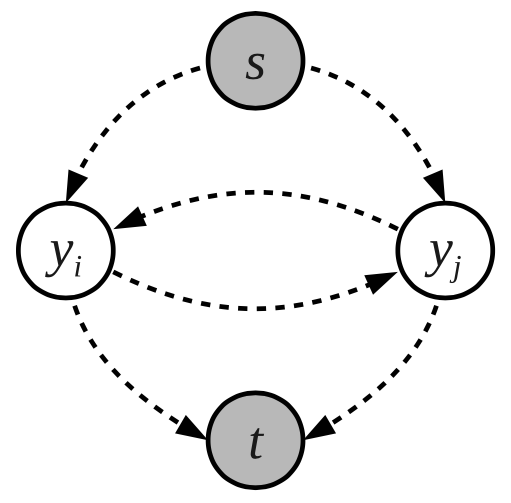
\includegraphics[width=0.5\columnwidth]{Methodology/figures/unary_pairwise.png}\\
  \caption{\label{fig:stmincut} $st$-graph
    construction~\cite{gouldlearning} for unary and pairwise
    terms.}
\end{figure}

The construction is explained in \figref{fig:stmincut}. It
denotes construction for unary and pairwise terms (see
\cite{Kolmogorov:PAMI04}). For unary edges (4 edges on both
sides), weights on each edge are corresponding to values in input
unary terms accordingly. For pairwise edges (2 edges in the
middle), both edges share the same weight which equals to the
input pairwise term. Every cut corresponds to an assignment to
the random variables, where variables associated with nodes in
the ${\cal S}$ set take the value one, and those associated with
nodes in the $\T$ set take the value zero. With slight abuse of
notation, we use the variables to denote nodes in our graph.



% %%% Local Variables:
% %%% mode: latex
% %%% TeX-master: "../thesis"
% %%% End:

